%==============================================================================
%% Template PROYECTO DE UTP
% Autor: Deybi Mojica
%        Lic.Ing. de Sistemas de Información       
%        Facultad de Ingeniera de Sistemas de Informción 
%        Universidad Tecnologica de Panamá
%==============================================================================
\documentclass[12pt,letterpaper,fleqn]{report}
\usepackage{UCM}
  
\begin{document}
\pagestyle{empty}
\begin{center}
    \parbox[c][\textheight][t]{\textwidth}{
        \begin{center}
            
\includegraphics[scale=0.05]{./figures/01-u.png}\\
            \vspace{0.25cm}
           {\normalsize \bf Universidad Tecnológica de Panamá}\\ \vspace{-0.15cm} 
                {\normalsize \bf Centro Regional de Chiriquí}\\ \vspace{-0.10cm}
            {\normalsize Facultad de Ingeniería Sistemas Computacionales}\\ \vspace{-0.15cm} 
            {\normalsize Carrera en Licenciatura en ingeniera en sistemas de Información}\\
            \vspace{2cm}
            {\normalsize \bf Proyecto de Evaluación de la cultura digital en Panamá y propuesta de un modelo de asistente para concientizar sobre navegación segura en internet.} \\
            \vspace{2cm}
            {\normalsize \bf Integrantes: } \\
            {\normalsize \bf Nefthaly Abrego } \\
            {\normalsize \bf Madeline De León} \\
            {\normalsize \bf Deybi Mojica    } \\ 
             \vspace{2cm}
            {\normalsize \bf Facilitador: Dr. Santiago Quintero} \\
            \vfill
            Proyecto de Investigación presentado en conformidad a los requisitos para la Jornada de Investigación Científica \\
            \vspace{0.5cm}
            David,Chiriquí,  Julio 2023
        \end{center}
        }
\end{center}

%\newpage

\cleardoublepage
%---------------------------------------------------------------------------
% Preamble
\pagenumbering{roman} 				% Begin Roman page numbering (i,ii,...)
%---------------------------------------------------------------------------
% Resumen
\chapter*{Resumen}
 \addcontentsline{toc}{chapter}{Resumen}
El proyecto consiste en el diseño de un asistente con la integración de NanoGPT.
El cual tiene como finalidad concientizar a la población en el tema: “Navegación segura en internet”. 
A todo esto, se utilizará la integración de un modelo que hace uso de un conjunto de datos clasificados y etiquetados por categoría de amenazas en la web y dispositivos digitales. El fin de esto es realizar la selección de datos, verdaderos y congruentes, que son procesados en el entrenamiento; De ese modo el entrenamiento crea un fichero .pt, que da un modelo como resultado. Al generar las preguntas al modelo GPT se logra que este clasifique e identifique patrones en la entrada y responda con la información relevante sobre seguridad. 
Cabe resaltar que se ha realizado una encuesta que nos muestra una población de 76 personas encuestadas. De ese modo el 34,2 por-ciento responde que su conocimiento es básico en seguridad informática, Ahora bien, nos da una disyuntiva ya que el 69.3 por-ciento, nos dice que no ha experimentado ningún robo personal o infección de malware. Del mismo modo el 77.6 por-ciento concluye que están de acuerdo con un modelo de asistente GPT para mejoras en seguridad y noticias a nuevas vulnerabilidades.

 \cleardoublepage
% Abstract
\chapter*{Abstract}
 \addcontentsline{toc}{chapter}{Abstract}
 The project consists of the design of a wizard with the integration of NanoGPT.
The purpose of which is to raise awareness among the population on the subject: "Safe Internet browsing".
To all this, we continued with the integration of a model that makes use of a series of data, which begins with the classification of text by category of threats on the web and digital devices. The purpose of this is to carry out the selection of data, true and congruent, in which it is in charge of tokenization; In this way the training creates a .pt file, which gives a model as a result. It should be noted that a survey has been carried out that shows us a population of 76 people surveyed. In this way, 34.2 percent respond that their knowledge is basic in computer security. However, it gives us a dilemma since 69.3 percent tell us that they have not experienced any personal theft or malware infection. In the same way, 77.6 percent conclude that they agree with a GPT assistant model for security improvements and news of new vulnerabilities.

 \cleardoublepage
%---------------------------------------------------------------------------
% Agradecimientos
% Se puede remover si el estudiante no lo desea (máximo una página)
%\chapter*{Agradecimientos}
%\addcontentsline{toc}{chapter}{Agradecimientos}
%\lipsum[5-6]

\cleardoublepage
%---------------------------------------------------------------------------
%The table of contents is automatically generated by the template
\setcounter{secnumdepth}{4}
\setcounter{tocdepth}{4}            % Sets the number of section levels in the table of contents to 4
\tableofcontents                    % Creates the table of contents
\cleardoublepage                    % Ends the current page

\listoffigures
\addcontentsline{toc}{chapter}{\listfigurename}
\cleardoublepage 
%\listoftables
%\addcontentsline{toc}{chapter}{\listtablename}
%\cleardoublepage 
%---------------------------------------------------------------------------
% Capitulos
\pagestyle{fancy}               	% Fancy headings
\pagenumbering{arabic}				% Begin arabic page numbering (1,2,...)
\setlength{\parindent}{20pt}        % Sets default paragraph indentation to 20 pt 
% Capítulos
\chapter{Introducción}\label{cap:capitulo_1}
%---------------------------------------------------------------------------
La sociedad actual, está completamente digitalizada, pero carece de conciencia digital que permite disminuir los riesgos: La falta de conocimiento relacionado con las tendencias actuales del Internet de las Cosas (IoT), las plataformas cloud, los servicios en la nube, las redes sociales y el uso de aplicaciones Fintech. (De este modo se atraen a los ciberdelincuentes para aprovecharse y ampliar su modus operandi). Aun así, toman ventaja de la información personal publicada en redes sociales, además de que utilizan ataques para intervenir y captar datos que pueden utilizar en contra de la víctima para sacar beneficio. Aun cuando son desplegadas y adoptadas estás tecnologías se requiere de un personal consiente como: primeria línea de defensa ante ataques; ya que los sistemas por si solos a pesar de contar con mecanismos de tecnologías preventivas y para la detección (son los usuarios los cuales manipulan, configuran y utilizan las tecnologías). \\

El creciente uso de los medios digitales en diversas áreas cotidianas de la vida ha hecho que los ciudadanos estén más conectados a lo que sucede en su entorno, estos utilizan tecnologías para comunicarse por múltiples medios sociales, controlar remotamente equipos, maquinarias y realizar transacciones. Este nuevo ecosistema digital donde concurren las interacciones sociales contiene una creciente ola de riesgos que pueden moldear el comportamiento en masa, influir, manipular y provocar daños con ataques en el ecosistema digital en la llamada nueva ciudadanía digital \cite{A2020}. \\

En necesaria para la sociedad en general que los desarrollos e implementaciones de tecnologías se orienten a innovaciones inclusivas que mejoren el bienestar social, algo que es un reto para países menos desarrollados en el ámbito cultural tecnológico creando brechas de conocimiento que provocan afectaciones en la seguridad personal, social, empresarial y nacional. Como lo menciona  \cite{Nadeesha2021}, casos como el ciberacoso, el fraude, suplantación de identidad, filtración de datos y perdidas, infiltración en sistemas críticos pueden generar caos social, por lo que es necesario educar desde temprano sobre seguridad cibernética, otros autores que han realizado investigaciones sobre conciencia digital han identificado los grupos de estudio tienen un bajo nivel de conocimiento sobre malwares, técnicas de phishing, ataques de fuerza bruta y uso de contraseñas inseguras \cite{Eslavova2019}. \\

Esta investigación busca conocer el nivel de conciencia sobre riesgos cibernéticos en un grupo focal y plantea una propuesta a través de un prototipo de asistencia por lenguaje natural a través de texto por medio de modelo GPT adoptado a pequeña escala y ajustado a temas de que apoyen a la concienciación sobre seguridad informática y navegación segura en internet.\\
 
\section{Formulación de hipótesis y objetivos} \label{section:thesis organization} % you can assign a unique label to each chapter or section for crossreferencing

    \begin{itemize}
        \item En Panamá existe conciencia sobre los riesgos y vulnerabilidades en el ciberespacio.
        \item Mediante un modelo GPT entrenado con un Dataset se puede dar un mejor enfoque para concientizar y comunicar las amenazas y brindar recomendaciones de mitigación.
        \item ¿Un asistente puede concienciar sobre la seguridad digital y sobre la importancia de la seguridad y del uso de técnicas que permitan aplicar buenas ‘prácticas de navegación en la sociedad informática en los medios electrónicos digitales?

    \end{itemize}

%/\subsection{This is a subsection}
 {\normalsize \bf Palabras Clave: }
    {\normalsize Asistente digital, Seguridad Informática, Modelo GPT, Cultura de seguridad digital.}

%---------------------------------------------------------------------------

%---------------------------------------------------------------------------         

\chapter{Marco Teórico}\label{cap:capitulo_2}
%---------------------------------------------------------------------------

\section{Cultura, sociedad y conciencia digital.}\label{section:Cultura, sociedad y conciencia digital.}
La ciudadanía digital es la adopción del uso de sistemas de información y tecnológico para la sociedad, a través de los cuales realizan transacciones diarias con su entorno. Esto permite que todos los ciudadanos puedan consumir y utilizar los servicios públicos a través de medios digitales\cite{Popkova2020}.
A medida que la sociedad y las ciudades pasan a un enfoque inteligente donde todo está digitalizado aumentan más los desafíos de seguridad protección y privacidad. Muchas ciudades utilizan medidores inteligentes, cámaras de vigilancia por internet, pagos de servicios públicos, redes wifi-nacionales que logran una conectividad y alcance mayor al acceso a internet. Toda la información generada en la sociedad está siendo digitalizada \cite{Konkolewsky2017}. \\
La ciudadanía digital se puede llevar a través de comunidades en internet en donde el individuo adquiere una identidad, derechos, obligaciones que hacen que su participación a través de esta sea válida para la interacción social con su entorno de forma libre\cite{Popkova2020}. \\
La conciencia digital es el punto de partida para una cultura digital sólida, diversos estudios demuestran que la capacitación sobre la seguridad informática es una excelente manera de comunicar y concientizar a la población sobre las amenazas digitales. En el estudio realizado por \cite{}, se demuestra esto a través de la investigación de un grupo de niños y jóvenes a los cuales se les proporcionó información sobre las amenazas en internet, casos de estudio e historias. Otros estudios demuestran como las empresas adoptan este sistema de capacitaciones para asegurar la infraestructura y sus activos para garantizar la continuidad y cultura empresarial digital logrando mitigar las amenazas cibernéticas con este enfoque. \cite{Li2021}\\
Al igual que una empresa, los países deben buscar proteger a los ciudadanos, los programas educativos, las implementaciones curriculares de tecnología permiten hacer que las generaciones venideras se conviertan en buenos ciudadanos digitales y usuarios de internet. Es complicado lograr esto en la práctica ya que, cada generación, grupo social, puede ser visto desde diferentes ángulos con respecto a el ámbito tecnológico, este aspecto generacional y profundización de internet en las generaciones venideras pueden hacerlas más propensas a engaños, perdida de sus datos y renuncia a su información con tal de aprovechar los beneficios de los servicios que utilizan\cite{Francis2022}. \\
%---------------------------------------------------------------------------
\section{Cultura digital y ciberseguridad en Panamá}\label{section:Cultura digital y ciberseguridad en Panamá}
En la investigación de \cite{Graell2022}, se indaga sobre el ciudadano panameño en aspectos de brechas digitales e informática educativa. En la investigación se realizó un proceso exploratorio para ver la adopción y cotidianidad de uso de tecnologías sobre materia digital. En Panamá se tiene un alcance de la red nacional de internet que permite cerrar brechas, pero aún existen retos para romper las desigualdades de acceso y participación a través de la red, algo se deslumbró con la pandemia como lo menciona \cite{} en la educación, en el acceso a la información por medios digitales obligados por la pandemia. Muchas de las instituciones han transformado sus servicios a enfoques digitales que permiten el rápido acceso a sus ciudadanos. Plataformas como Panamá Digital y muchas otras implementaciones a nivel educativo han aumentado la forma en que la sociedad interactúa con las instituciones educativas, financieras etc. Los retos de las brechas sociales y las capacidades relacionadas para crear conciencia digital entre diversas culturas internas, grupos sociales dificultan la capacitación a nivel de País para mitigar problemas y afectaciones a ciudadanos con carentes conocimientos que acceden a estas plataformas de instituciones públicas. Según \cite{Graell2022}, el ciudadano digital debe poseer educación en tecnología, estándares de conducta en medios electrónicos, participación electrónica, responsabilidad, libertades e inclusión, conciencia digital sobre los riesgos. Este conjunto de capacidades del ciudadano digital hace que este posea capacidad para actuar con conciencia y libertad siendo responsabilidad sobre los medios digitales, este espacio de sociedad virtual y cultura permite que los ciudadanos mantengan estándares de conducta y conciencia que permite la paz social resultado del buen el uso de la tecnología. \\
Por otro lado, según la AIG, en Panamá no se escapa de los ciberataques, en el 2021 se registraron en el País más de 3.2 millones de intentos, durante la pandemia las cifras aumentaron por el trabajo remoto, las clases en línea, pagos a empresas a través de medios virtuales etc. Estas cifras colocan a Panamá en el top 10. Si las empresas, personas y el gobierno no implementan medidas y una cultura de ciberseguridad estos ataques pueden generar alteración en la vida cotidiana y en la sociedad \cite{AIG2022}.

%---------------------------------------------------------------------------
\section{ Delitos informáticos en Panamá y leyes}\label{section:Delitos informáticos en Panamá y leyes}
En Panamá existen leyes que determinan claramente los delitos cibernéticos como se menciona en el TITULO VIII del Código Penal sobre los delitos contra la seguridad jurídica de los medios electrónicos. En él se mencionan los delitos contra la seguridad informática y otros cuatro artículos,289,290,291 y 292. \\
Estas leyes apoyan las garantías constitucionales o legales en Panamá y penalizan o sancionan a aquellos que ejecuten actos delictivos por medios electrónicos o tecnológicos. Sin embargo, la sociedad no tiene cultura de denuncia cuando se es víctima de estos actos delictivos y las leyes actuales no persiguen estos delitos verdaderamente \cite{Francis2022}.

%---------------------------------------------------------------------------
\section{Revisión de la literatura}\label{section: Revisión de la literatura}
\subsection{Asistentes digitales}
Los asistentes digitales se han implementado en muchas industrias, empresas, departamentos para establecer conversaciones con las personas. Estos asistentes son capaces de comprender la entrada del usuario y responder bajo el contexto. La inteligencia artificial ha empoderado a estos asistentes haciéndolos más robustos y fuertes para mantener la interacción \cite{Urribarri2022}.
\subsection{Procesamiento del lenguaje natural e inteligencia artificial}\label{section: NPT e IA}
En los últimos años hemos visto como la disciplina aplicada de la inteligencia artificial han incrementado los casos de uso y beneficiado a múltiples sectores haciendo que se mejore la capacidad de análisis y procesamiento con inteligencia que simula a la humana. Los asistentes virtuales con IA es uno de estos casos de uso en donde se aplica tecnología de procesamiento de lenguaje natural; esta técnica permite que un equipo computacional pueda analizar e interpretar el idioma humano a través de algoritmos que permiten realizar procesos para comprender las estructuras textuales. Esta área es un subconjunto de técnicas utilizadas para generar algoritmos de inteligencia artificial que se acerquen a las capacidades humanas. La inteligencia artificial en general propone muchas oportunidades de aplicación en contextos de la vida diaria.
\subsection{Modelos y herramientas para generar conversaciones fluidas}\label{section: Modelos y herramientas}
Los modelos transformadores generativos pre-entrenados(GPT) utilizan técnicas de aprendizaje profundo, procesamiento del lenguaje natural con redes neuronales   para la creación de texto, imágenes, voz, análisis y clasificación. Cuando son utilizados para la generación de texto, estos se basan en conocimientos que adquieren durante un entrenamiento con grandes cantidades de datos lingüísticos. 
Durante el proceso de codificación del texto de entrada (encoder) se crea una representación numérica vectorial que puede ser procesada por la máquina para posteriores decodificaciones, durante este proceso el texto es dividido en partes llamadas tokens los cuales son vectorizados y dados de entrada a la red neuronal.
Cuando se inicia el proceso de entrenamiento la red neuronal ajusta sus pesos como perillas que ajustan probabilísticamente el modelo para dar el texto más acorde a la secuencia de palabras.\cite{Alex2023}, \cite{AWS2022}

El creciente uso de los modelos de lenguaje natural ha mejorado y dado muchas aplicaciones prácticas de procesamiento del lenguaje natural. Estos modelos requieren un corpus de texto de entrenamiento seguido de ajustes que permitan ajustar el modelo para responder y realizar tareas específicas, el modelo GPT-3 tiene 175 mil millones de parámetros y fue entrenado con un amplio contenido de texto web \cite{Brown2020}. 
Existen marcos de trabajo configurables que permiten crear soluciones GPT rápidamente, una de estas es nanoGPT que admite crear modelos con grandes cantidades de parámetros como GPT-2, desde una estructura de código limpia y de pocas líneas. 
%---------------------------------------------------------------------------
\section{Estudios relacionados}\label{section: Estudios relacionados}
La inteligencia artificial y sus sub-ramas proponen aplicaciones que pueden ser orientarse a soluciones para generar más inclusión social y desarrollo cultura de un país. \\
Actualmente no hay estudios que basen modelos de asistentes orientados en la asistencia a la educación sobre ciberseguridad y conciencia digital. Los estudios relacionados se basan en modelos orientados a asistentes comerciales como el realizado por \cite{VarelaTapia2022}, que implemento un sistema web basado en plataforma DialogFLow que trabaja con el modelo BERT para interpretar el texto, consistió en un asistente web para apoyo a la atención al cliente a través de una interfaz web. El estudio muestra una arquitectura de cliente servidor que permite a través de una interfaz interactuar con el cliente final para responder preguntas relacionadas al comercio. El estudio muestra como el modelo de DialogFlow permite utilizar los algoritmos de NPL para responder a preguntas no establecidas previamente, al estar utilizando modelos NPL se puede interpretar la pregunta del usuario y que el modelo responda con base a el conjunto de datos con el que fue entrenado.
%---------------------------------------------------------------------------
\section{Objetivos del proyecto}\label{section:Objetivos del proyecto}
\subsection{Objetivo general}\label{section:Objetivo general}
Evaluar el nivel de conciencia digital en Panamá mediante la propuesta  de un prototipo de asistente digital basado en un modelo GPT, entrenado con datos sobre seguridad informática.
\subsection{Objetivos específicos}\label{section:Objetivos especificos}
 \begin{enumerate}
        \item Construir del conjunto de datos de entrenamiento relacionado a vulnerabilidades comunes, consejos de mitigación y de buenas prácticas de navegación y uso de medios digitales.
        \item Ajustar un modelo GPT mediante la utilización del conjunto de datos para asistir con respuestas relevantes sobre seguridad informática, consejos de mitigación de vulnerabilidades, buenas prácticas de navegación.
        \item Entrenar el modelo GPT, utilizando un conjunto de datos optimizados, relacionados a los riesgos de la navegación en Internet. 
    \end{enumerate}
    
%---------------------------------------------------------------------------
 

\chapter{Materiales y Métodos}\label{cap:capitulo_3}
%---------------------------------------------------------------------------
\section{Materiales y métodos para la recolección de datos y análisis de la población.}\label{section:Materiales y métodos para la recolección de datos y análisis de la población } 
Para el proyecto se realiza la validación de la conciencia digital sobre la navegación segura en internet en un grupo aleatorio aplicando una encuesta para la recolección de los datos que permiten validar o descartar la primera hipótesis. La encuesta busca evaluar el nivel de conocimiento sobre la navegación y seguridad en el ciberespacio en un grupo aleatorio de personas con datos básicos sobre la edad y el nivel de conocimiento en tecnología, además. Se realiza un muestreo aleatorio simple aplicado en el distrito de David cabecera, Chiriquí. \\
Las preguntas de la encuesta se orientaron a identificar el nivel de conciencia digital y conocimiento sobre  Malware, uso de métodos de seguridad y conocimiento sobre identificación de amenazas. \\
Para la selección de la muestra se consideró un subconjunto de la población finita de 96321 habitantes. Dato identificado en las estadísticas del INEC \cite{INEC}. \\
Los datos recopilados se analizarán con estadística descriptiva y permitirán validar o desechar la primera hipótesis. \\
Por lo tanto, realizando el muestreo con la población tenemos una muestra con un margen de error del 10\% como rango para reflejar la variación de los resultados de la población general, un nivel de confianza del 95\% para reflejar las actitudes más precisamente. Al calcular el tamaño de la muestra se obtiene el tamaño de 96 participantes que serán seleccionados aleatoriamente. \\
Para la escala de medición se aplican niveles de ponderación sobre las preguntas relacionadas a prácticas de seguridad online, en donde 1 es falta de conciencia y métodos de navegación segura, 2 uso medio de métodos seguros y conciencia media, 3 conocimiento de los riesgos y uso de mecanismos de seguridad.
%---------------------------------------------------------------------------
\section{Metodología y materiales para el desarrollo del modelo GPT.}\label{section:Metodología y materiales para el desarrollo del modelo GPT} 
Luego de la aplicación de la encuesta se realiza la recopilación de un conjunto de datos sobre buenas prácticas de navegación, consejos clasificados y etiquetados por categoría de amenazas en la web que luego son procesados para crear subconjuntos de entrenamiento y validación.
Para la construcción del modelo se utiliza el framework NanoGPT, esta es una solución a pequeña escala que permite reproducir modelos GPT simples y complejos entrenamientos con pocas líneas de código. \cite{Yang2020}
Para ello se realizan las etapas siguientes:
 \begin{itemize}
        \item 1.    Creación del conjunto de datos etiquetados
        \item 2.	Carga y preparación del conjunto de datos nanoGPT
        \item 3.	Entrenamiento
        \item 4.	Pruebas del modelo
    \end{itemize}
%---------------------------------------------------------------------------

%--------------------------------------------------------------------------- 

%\chapter{Desarrollo de propuesta de prototipo}\label{cap:capitulo4}

%---------------------------------------------------------------------------
\subsection{Creación de conjunto de datos de entrenamiento y adaptación de nanoGPT}\label{section:Creación de conjunto de datos con fuentes de internet} 
El conjunto de datos contiene recomendaciones y prácticas de seguridad clasificadas por categorías como amenazas, ataques y malware, figura \ref{figure:Conjunto de datos}. Esta clasificación permite que el modelo mejore clasifique mejor la entrada de texto dada.
\begin{figure}[H]
   \centering % figure is centered on the page
       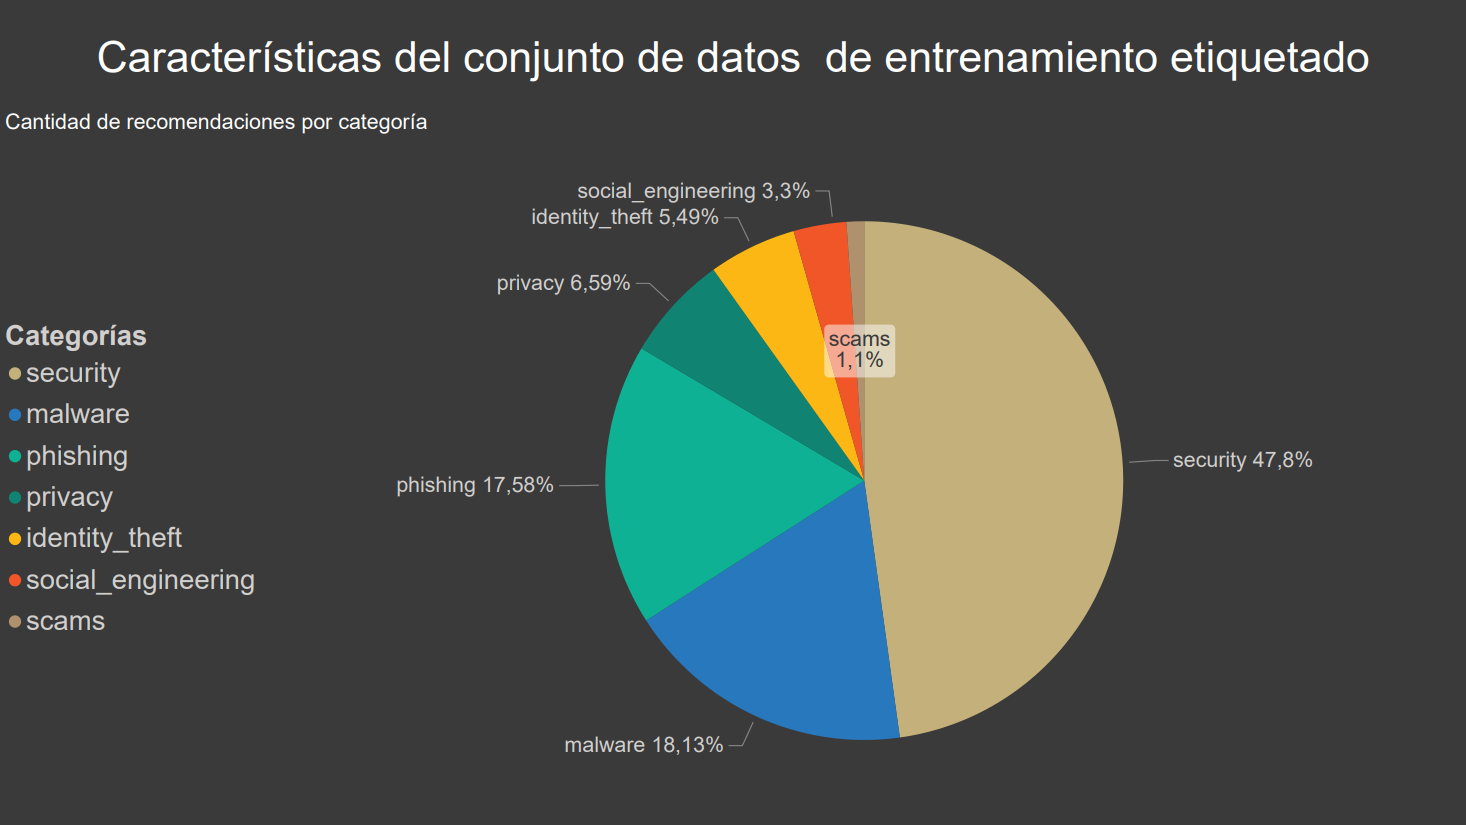
\includegraphics[width=0.6\linewidth]{./doc/Conjunto de datos etiquetado.png} 
   \caption{Características del conjunto de datos etiquetados \cite{}}
  \label{figure:Conjunto de datos}  % assign a unique label to each figure 
\end{figure}
%---Parrafo
Este se extrae desde el archivo CSV con el uso de la librería pandas a un dataframe. Figura \ref{figure:Extracción de datos del csv}.\cite{Reiss2021}
\begin{figure}[H]
   \centering % figure is centered on the page
       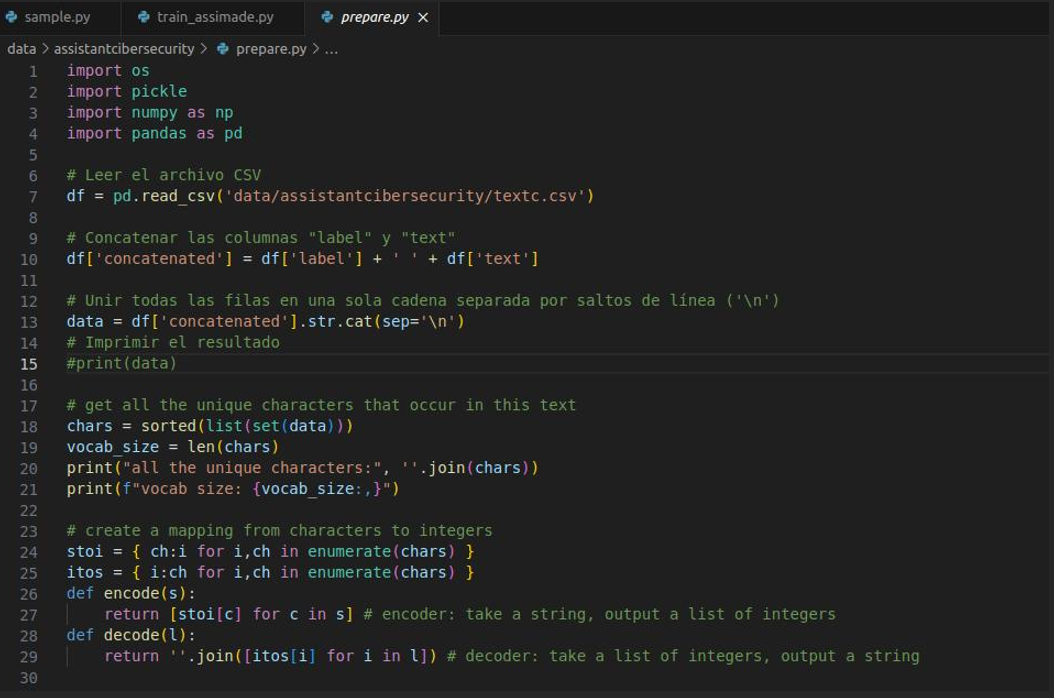
\includegraphics[width=0.6\linewidth]{./doc/02-cr.png} 
   \caption{Configuración para extraer el conjunto de datos en un dataframe y preparación de los datos.  \cite{}}
  \label{figure:Extracción de datos del csv}  % assign a unique label to each figure 
\end{figure}
Para el entrenamiento con NanoGPT se crean las carpetas del conjunto de datos, se realiza el proceso de mapeo de caracteres a enteros también llamado vectorización para representar los datos de texto en secuencias de números. \cite{GenerGediz2020}
En la figura \ref{figure:Etapa de encoder}
\begin{figure}[H]
   \centering % figure is centered on the page
       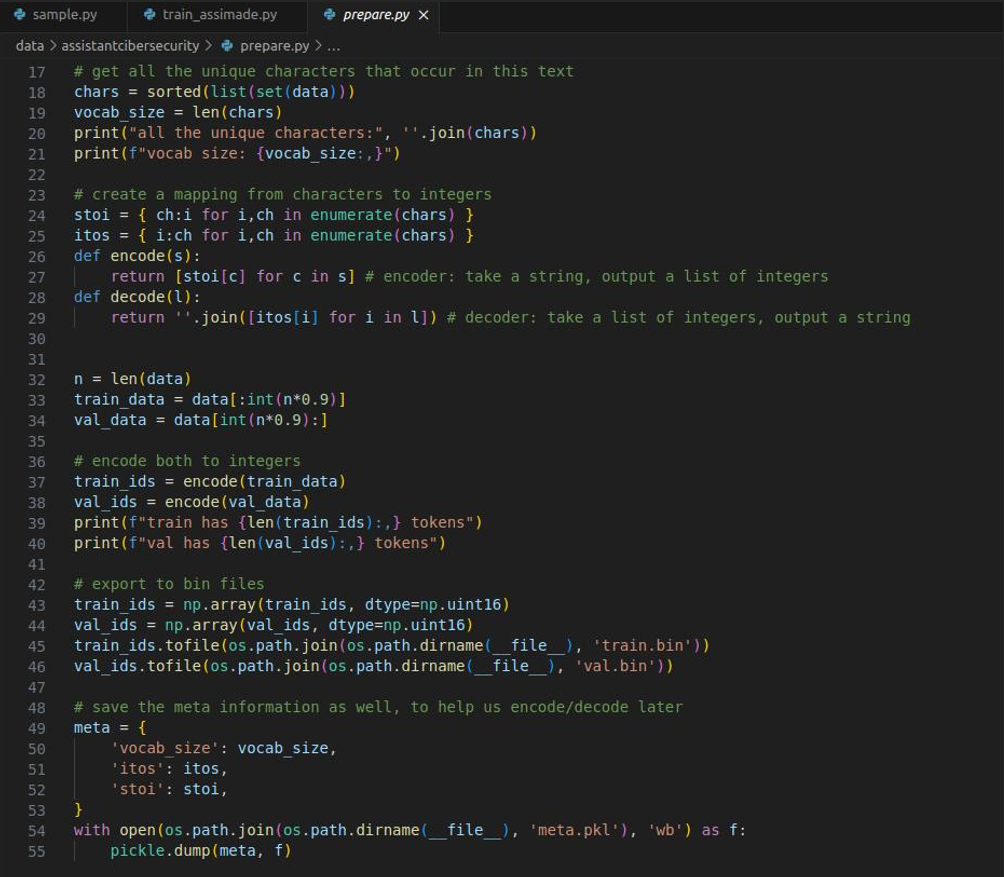
\includegraphics[width=0.6\linewidth]{./doc/03-cr.png} 
   \caption{procesamiento crea  ficheros de validación, entrenamiento y un meta modelo de apoyo.  \cite{}}
  \label{figure:Etapa de encoder}  % assign a unique label to each figure 
\end{figure}
%Parrafo-----
El procesamiento anterior crea ficheros de validación, entrenamiento y uno que contiene metadatos de los diccionarios para transformar de índices a palabras y viceversa para apoyo al proceso de condificación y decodificación.
\begin{figure}[H]
   \centering % figure is centered on the page
       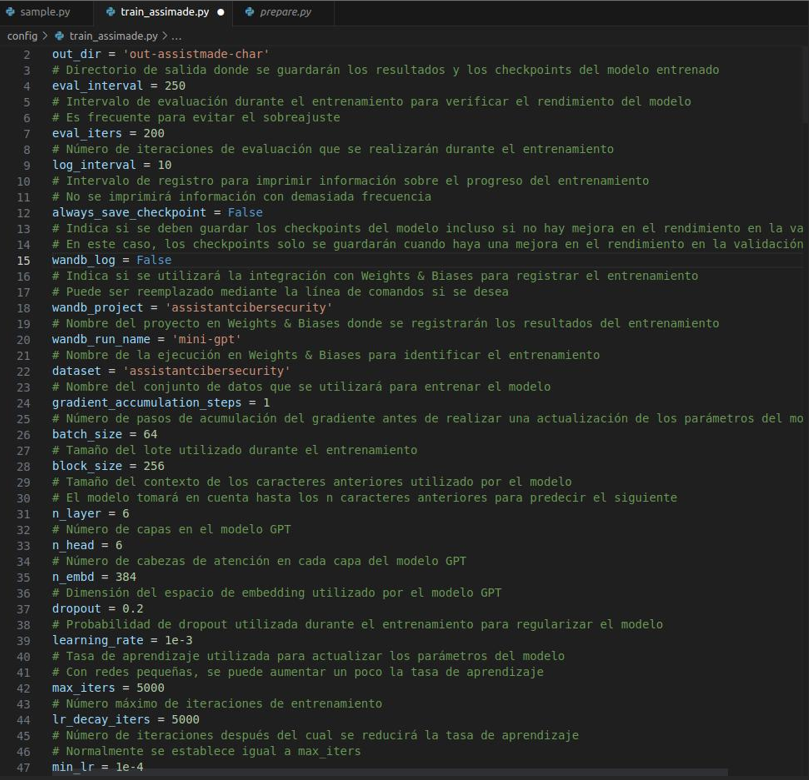
\includegraphics[width=0.8\linewidth]{./doc/04-cr.png} 
   \caption{Configuraciones y parámetros de entrenamiento que crea los directorios de salida para el modelo entrenado.  \cite{}}
  \label{figure:Configuraciónes de parámetros}  % assign a unique label to each figure 
\end{figure}
\clearpage
%---------------------------------------------------------------------------
\subsection{Configuración de los parámetros del código y entrenamiento}\label{section:Configuración y entrenamiento} 
Posteriormente se configuran dos modelos de prueba con variaciones de parámetros basados intervalos de entrenamiento, tamaños de bloque de texto procesado, cantidad de lotes en paralelo, ciclos de entrenamiento. 
Estas se realizado sobre la CPU, por lo que las configuraciones están centradas en entrenamientos de bajo rendimiento, el propósito es verificar configuraciones que permitan al modelo clasificar la entrada de texto y el conjunto entrenado.
\begin{enumerate}
	\item El tamaño de lote permite configurar cantidad de ejemplos que se procesan de forma paralela.
	\item Tamaño en bloques de permite configurar la dimensión del vector que representa al texto ingresado de forma secuencial.
	\item Configuración de las número de capas de la red y número de capas de atanción por cada capa de la red neuronal.
	\item Los vectores de incrustación para representar las palabras numéricamente vectores y generar resultados relacionados.
	\item Configuración de la red neuronal a 4 capas y 4 capas de atención que dan al modelo capacidad para asignar pesos del entrenamiento. 
	\item El tamaño de los vectores permiten crear una mayor representación de cantidades de palabras en la oración  para identificar representaciones significativas en un texto transformado.
	\item Por último el parámetro para establecer las iteraciones de entrenamiento se establecen en 3000. 
\end{enumerate} 
\begin{table}[H]
	\centering
	\begin{tabular}{|c|c|c|c|c|c|c|c|}
		\hline
		\textbf{Configuración} & \textbf{log\_interval} & \textbf{block\_size} & \textbf{batch\_size} & \textbf{n\_layer} & \textbf{n\_head} & \textbf{n\_embd} & \textbf{max\_iters} \\
		\hline
		Configuración 1 & 1 & 64 & 12 & 8 & 8 & 128 & 1000 \\
		Configuración 2 & 5 & 128 & 32 & 4 & 4 & 256 & 3000 \\
		\hline
	\end{tabular}
	\caption{Configuraciones de los modelos}
	\label{tab:configuraciones}
\end{table}
\subsection{Configuración 1}\label{section:Configuración de los parámetros del código} 
\begin{itemize}
	\item   Objetivo: Con esta configuración se busca mayor cantidad de parámetros el modelo reduciendo de bloque además se aumenta cantidad de capas de red y capas de atención.
\end{itemize}
\begin{figure}[H]
	\centering % figure is centered on the page
	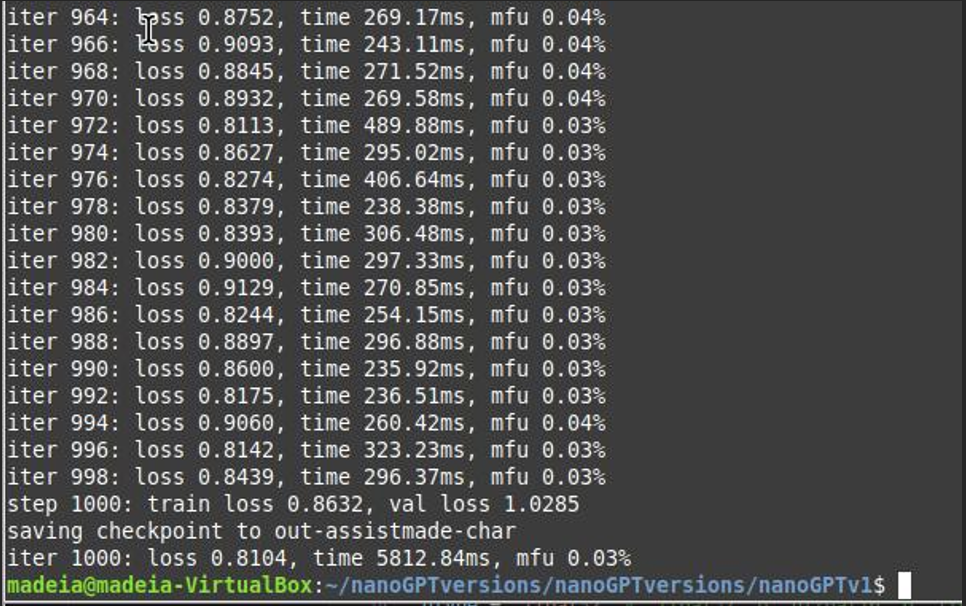
\includegraphics[width=0.65\linewidth]{./rp/15-cp.png} 
	\caption{Proceso de entrenamiento de modelo 1\cite{}}
	\label{figure:Resultado 1}  % assign a unique label to each figure 
\end{figure}
%------------------------------------------------------------------------------
\subsection{Configuración 2}\label{section:Configuración de los parámetros del código} 
\begin{itemize}
	\item   Objetivo: Esta configuración se centra en aumentar los lotes y capacidad de los bloques, se disminuyen las capas de la red y se incrementan los intervalos de evaluación ademas de la cantidad de iteraciones.
\end{itemize}
\begin{figure}[H]
	\centering % figure is centered on the page
	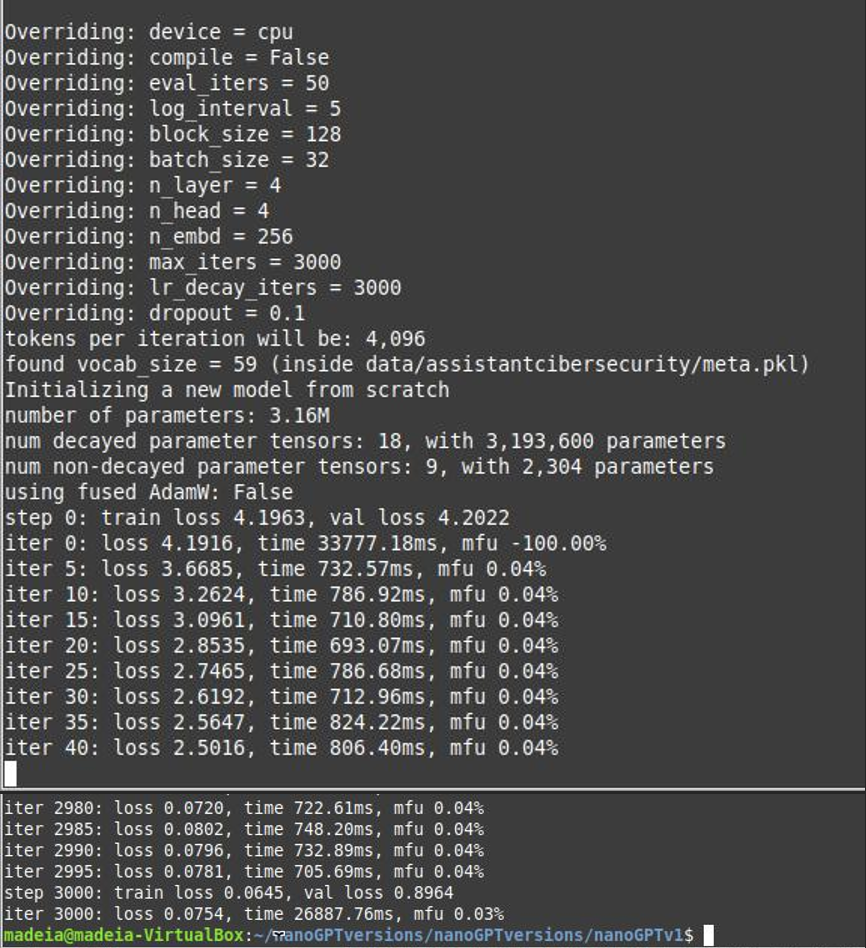
\includegraphics[width=0.65\linewidth]{./rp/05-cp.png} 
	\caption{Configuraciones de entrenamiento de modelo 2  \cite{}}
	\label{figure:Resultado 1}  % assign a unique label to each figure 
\end{figure}
\begin{figure}[H]
	\centering % figure is centered on the page
	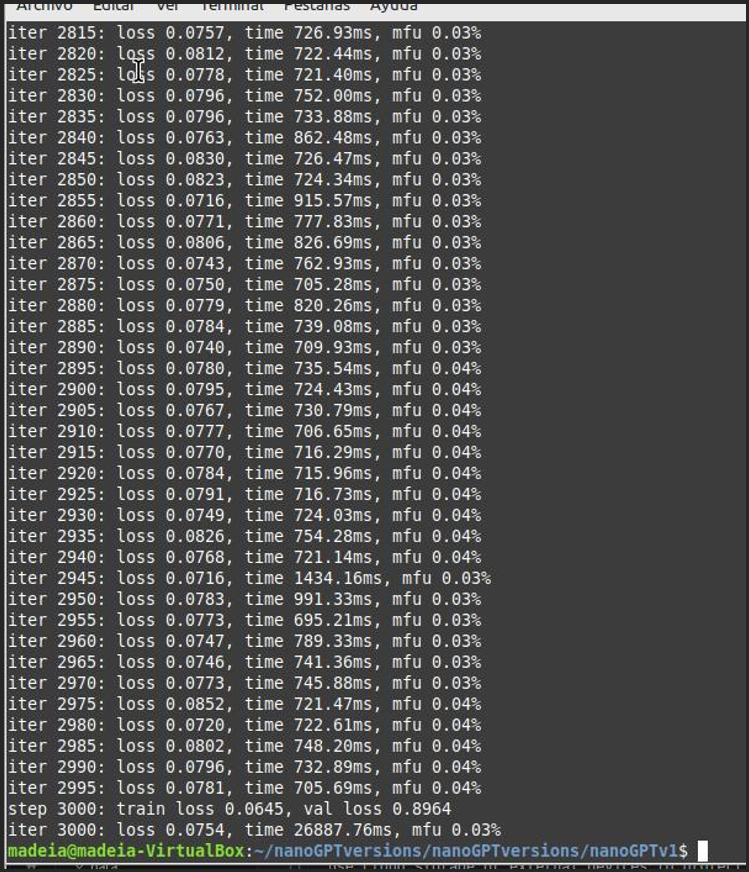
\includegraphics[width=0.65\linewidth]{./rp/06-cp.png} 
	\caption{Proceso de entrenamiento de modelo 2\cite{}}
	\label{figure:Resultado 1}  % assign a unique label to each figure 
\end{figure}


%-------------------------------------------------------------------------------
%------------------------------------------------------------------------------

\subsubsection{Configuración parámetros para entrenamiento}\label{section:Configuración de los parámetros del código} 
En la figura \ref{figure:Configuraciones modelo entrenamiento 2} se asignan a los parámetros mediante la ejecución del entrenamiento con en remplazo de las variables. Esto se realiza ejecutando el python y asignando los valores de las variables al ejecutar el archivo de entrenamiento.

\begin{figure}[H]
   \centering % figure is centered on the page
       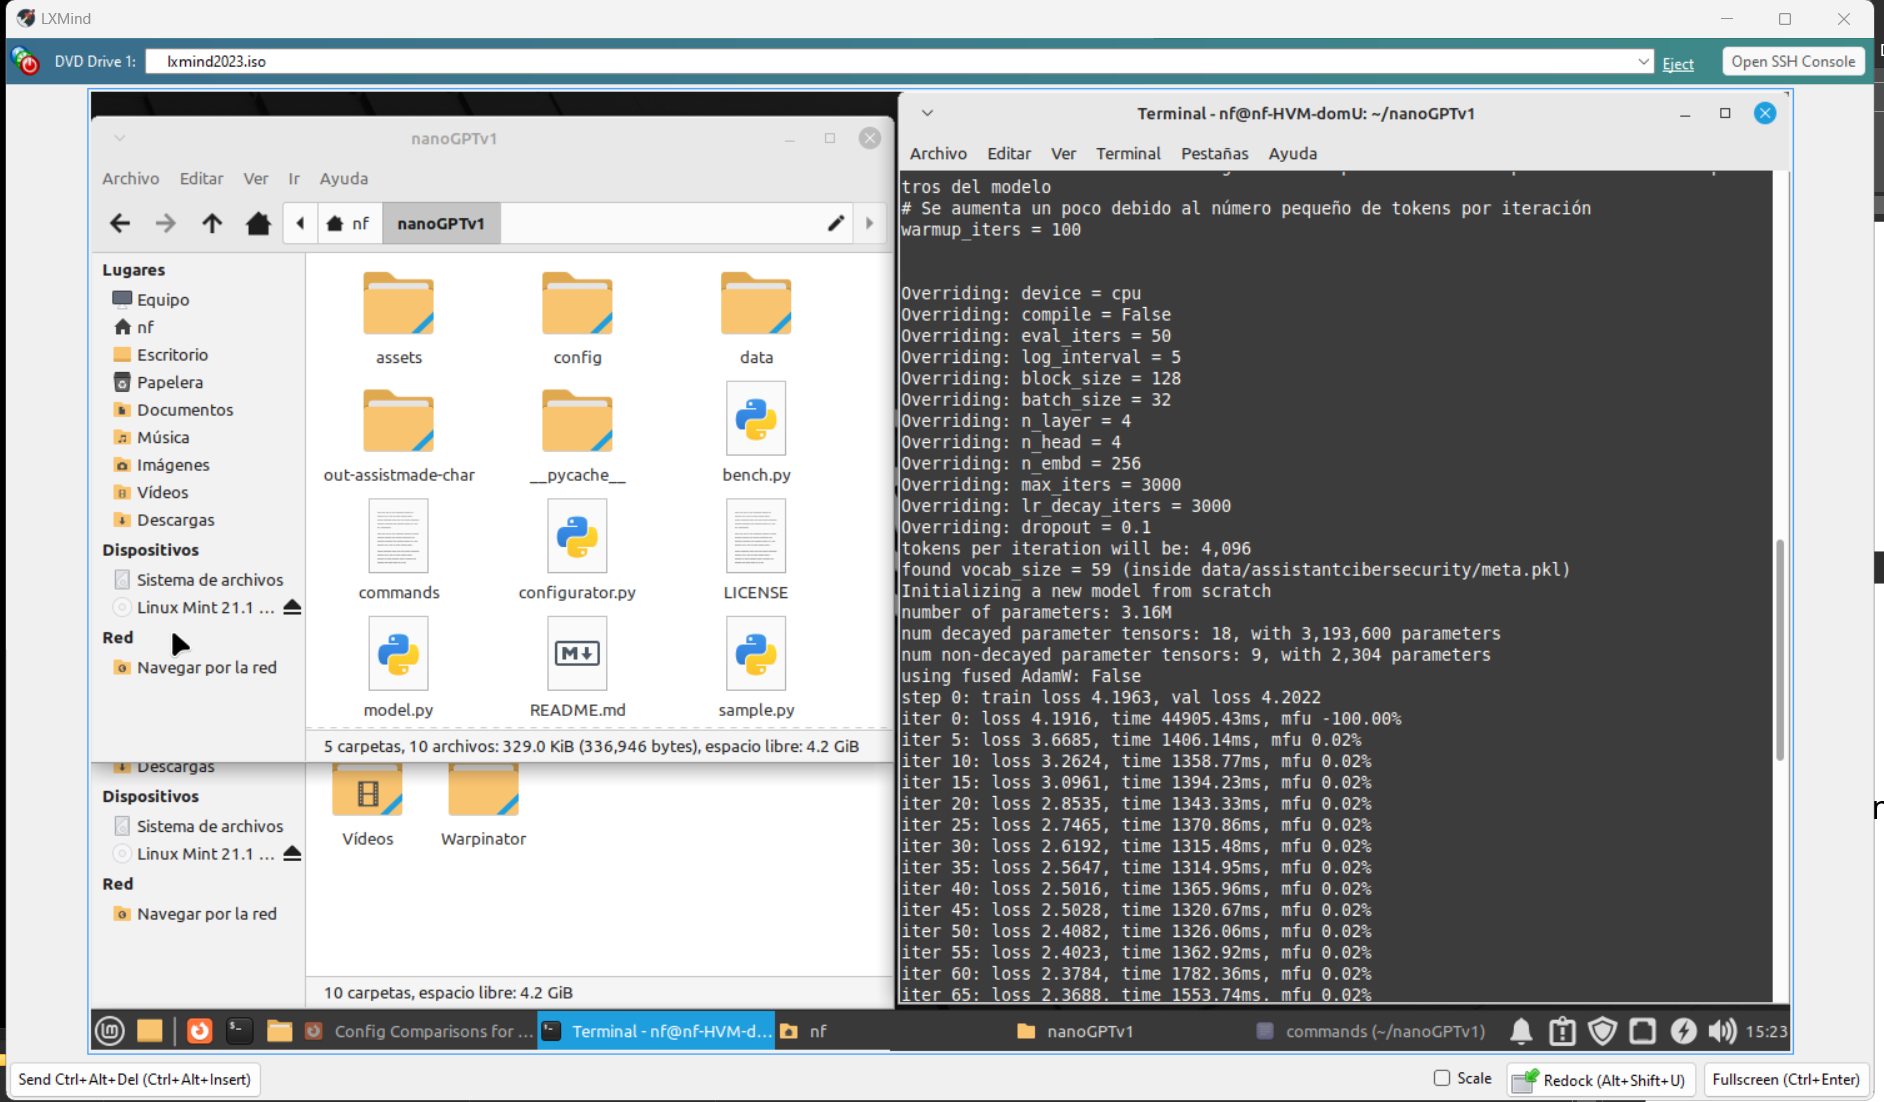
\includegraphics[width=0.7\linewidth]{./doc/Proceso de entrenamiento en XCP-ng.png} 
   \caption{Configuraciones de entrenamiento de modelo  \cite{}}
  \label{figure:Configuraciones modelo entrenamiento 2}  % assign a unique label to each figure 
\end{figure}
\begin{figure}[H]
   \centering % figure is centered on the page
       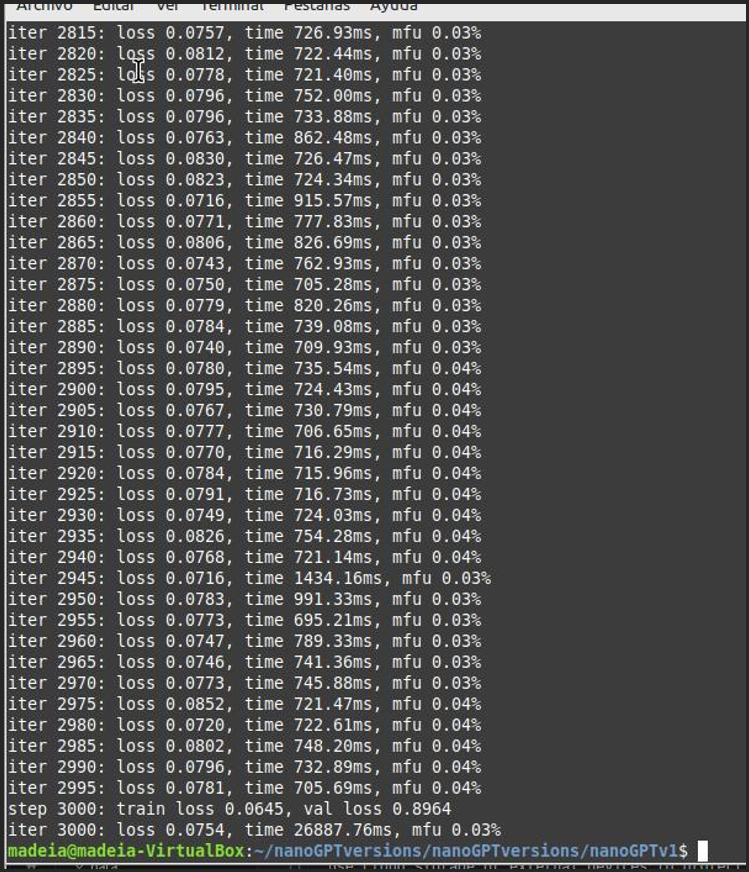
\includegraphics[width=0.5\linewidth]{./rp/06-cp.png} 
   \caption{Proceso de entrenamiento de modelo\cite{}}
  \label{figure:Proceso de entrenamiento del modelo}  % assign a unique label to each figure 
\end{figure}
%----------------------------------------------------------------------------
\clearpage

\subsection{Validación del modelo Configuración}\label{section:Validación de prompt}
\subsubsection{ Prueba 1}\label{section:Validación del prototipo}
Durante la prueba 1 se mantienen las configuraciones para ob
    \begin{itemize}
        \item   Top de tokens mas probables = 100
        \item   Temperatura = 1.2
        \item   Cantidad de tokens generados = 500
        \item   Prueba = python3 sample.py --out-dir=out-assistmade-char --device=cpu --start=" phising protection tips"
    
\begin{figure}[H]
   \centering % figure is centered on the page
       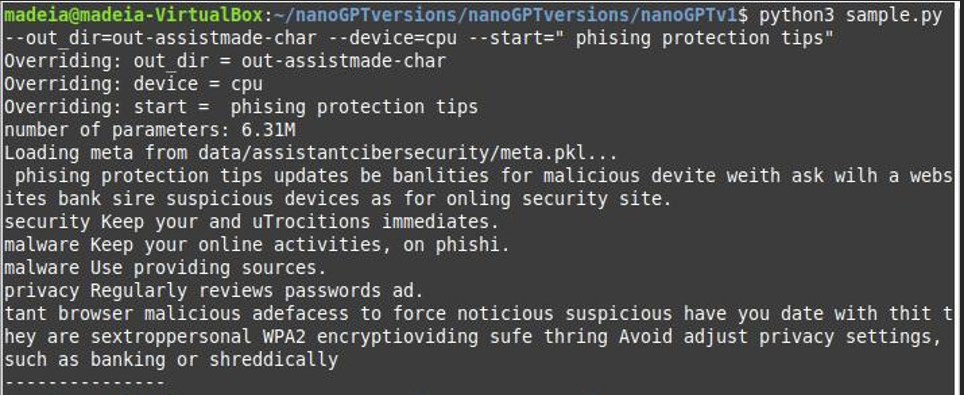
\includegraphics[width=0.65\linewidth]{./rp/16-cp.png} 
   \caption{Resultados de la Prueba 1\cite{}}
  \label{figure:Prueba1}  % assign a unique label to each figure 
\end{figure}
        \item   Prompt = python3 sample.py --out-dir=out-assistmade-char --device=cpu --start="safe internet browsing "
\begin{figure}[H]
   \centering % figure is centered on the page
       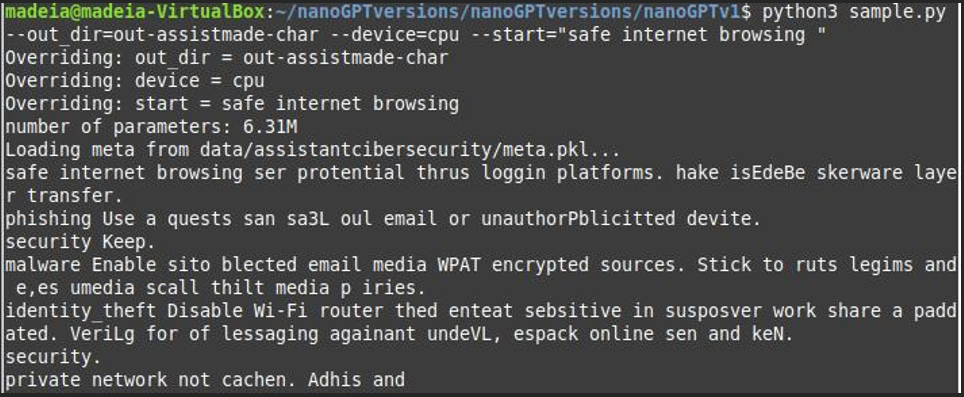
\includegraphics[width=0.65\linewidth]{./rp/17-cp.png} 
   \caption{Resultados de la Prueba 2\cite{}}
  \label{figure:Prueba2}  % assign a unique label to each figure 
\end{figure}
        \item   Prompt = python3 sample.py –out-dir=out-assistmade-char --device=cpu --start="computer security tips"
\begin{figure}[H]
   \centering % figure is centered on the page
       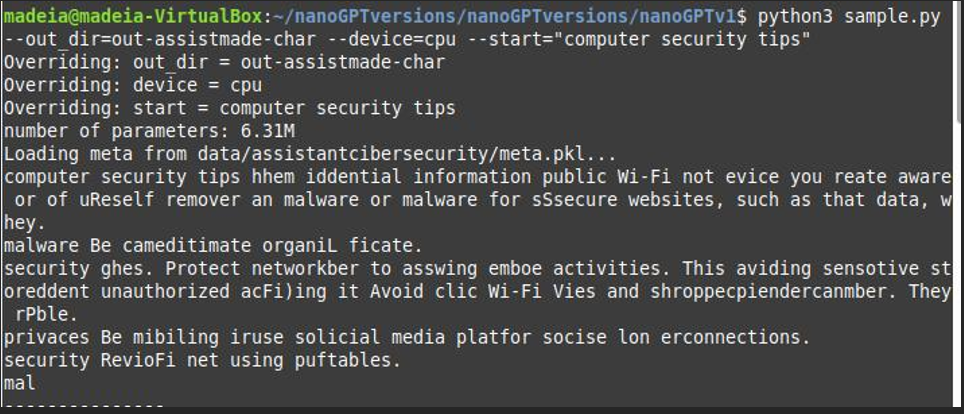
\includegraphics[width=0.65\linewidth]{./rp/18-cp.png} 
   \caption{Resultados de la Prueba 3\cite{}}
  \label{figure:Resultado prueba 3}  % assign a unique label to each figure 
\end{figure}
        \item   Prompt = python3 sample.py --out-dir=out-assistmade-char --device=cpu --start="prevent identity theft"
\begin{figure}[H]
   \centering % figure is centered on the page
       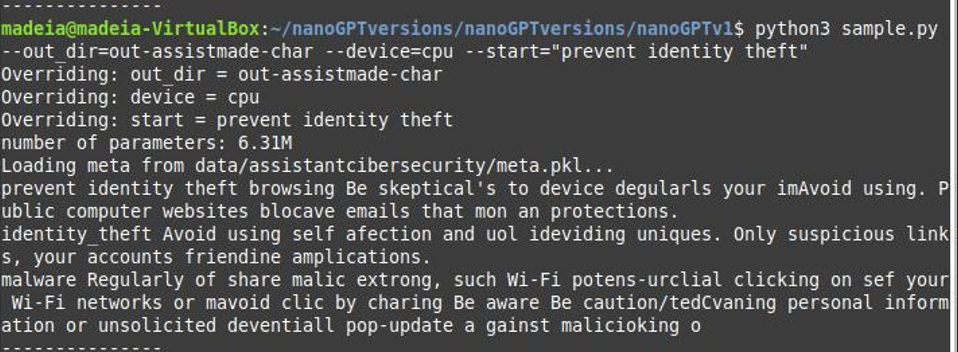
\includegraphics[width=0.65\linewidth]{./rp/19-cp.png} 
   \caption{Resultados de la Prueba 4\cite{}}
  \label{figure:Resultado prueba 4}  % assign a unique label to each figure 
\end{figure}
\end{itemize}
%-----------------------------------------------------------------------------   
\subsection{Validación del modelo Configuración 2}\label{section:Validación Modelo 2}
\subsubsection{ Prueba 1}\label{section:Prueba 1 config 2}
    \begin{itemize}
        \item   Top-k = 1
        \item   Temperatura = 10
        \item   Ma-new-tokens = 500
        \item    Prompt = python3 sample.py --out-dir=out-assistmade-char --device=cpu --start=" phising protection tips"
    \end{itemize}
\begin{figure}[H]
   \centering % figure is centered on the page
       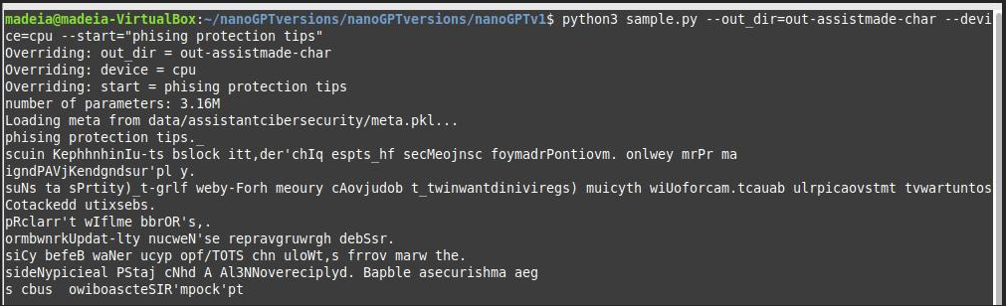
\includegraphics[width=0.65\linewidth]{./rp/07-cp.png} 
   \caption{Resultados de la Prueba 1\cite{}}
  \label{figure:Result prueba 1 mol 2}  % assign a unique label to each figure 
\end{figure}
\subsubsection{ Prueba 2}\label{section:Prueba2}
    \begin{itemize}
        \item   Top-k = 0.8
        \item   Temperatura = 10
        \item   Ma-new-tokens = 500
        \item   Prompt = python3 sample.py --out-dir=out-assistmade-char --device=cpu --start="safe internet browsing"
    \end{itemize}
\begin{figure}[H]
   \centering % figure is centered on the page
       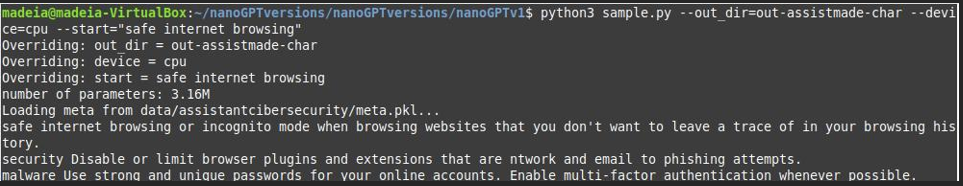
\includegraphics[width=0.65\linewidth]{./rp/08-cp.png} 
   \caption{Resultados de la Prueba 2\cite{}}
  \label{figure:Result prueb 2 mol 2}  % assign a unique label to each figure 
\end{figure}
\subsubsection{ Prueba 3}\label{section:Prueba 3 mol 2}
    \begin{itemize}
        \item   Top-k = 100
        \item   Temperatura = 1.2
        \item   Ma-new-tokens = 500
            \item   Prompt = python3 sample.py --out-dir=out-assistmade-char --device=cpu --start=" phising protection tips"
            \begin{figure}[H]
              \centering % figure is centered on the page
                  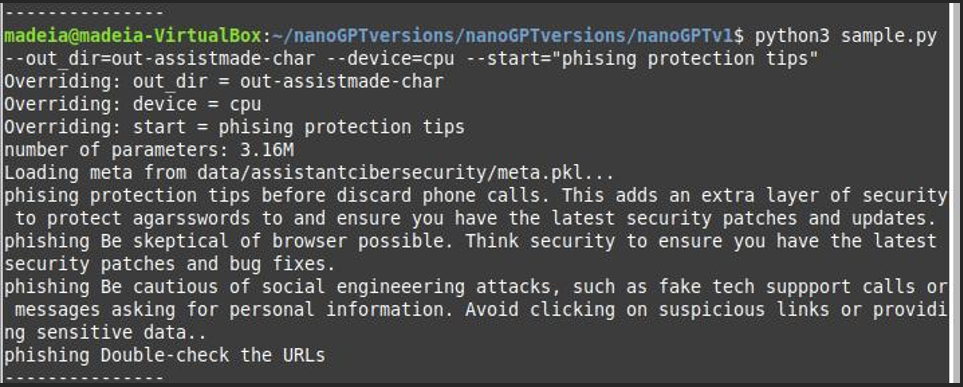
\includegraphics[width=0.65\linewidth]{./rp/09-cp.png} 
              \caption{Resultados de la Prueba 3.1\cite{}}
            \label{figure:Result Prueba 3 mod 2}  % assign a unique label to each figure 
            \end{figure}
            \item   Prompt = python3 sample.py --out-dir=out-assistmade-char --device=cpu --start="safe internet browsing"
            \item   Prompt = python3 sample.py --out-dir=out-assistmade-char --device=cpu --start="computer security tips"
            \begin{figure}[H]
              \centering % figure is centered on the page
                  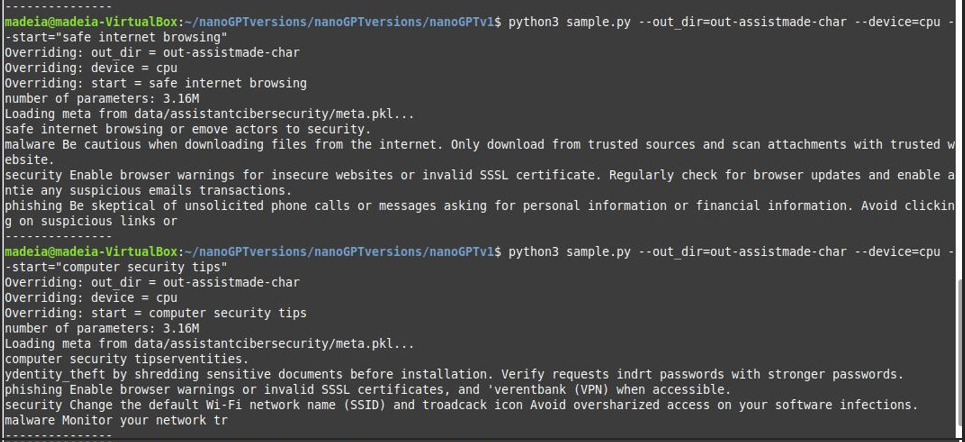
\includegraphics[width=0.65\linewidth]{./rp/10-cp.png} 
              \caption{Resultados de la Prueba 3.2 y 3.3\cite{}}
            \label{figure:Resultado 3.2}  % assign a unique label to each figure 
            \end{figure}
            \item   Prompt = python3 sample.py --out-dir=out-assistmade-char --device=cpu --start="computer security tips"
            \begin{figure}[H]
              \centering % figure is centered on the page
                  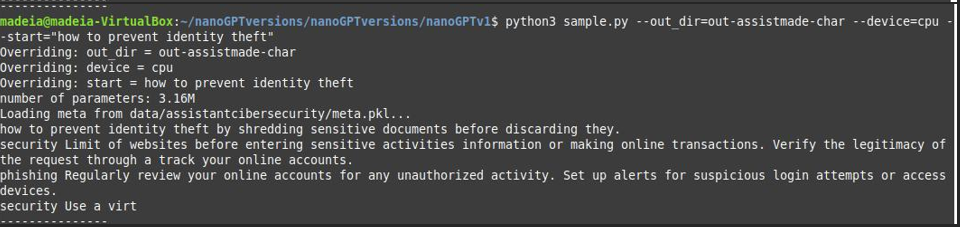
\includegraphics[width=0.65\linewidth]{./rp/11-cp.png} 
              \caption{Resultados de la Prueba 3.4\cite{}}
            \label{figure:Resultado 3.4}  % assign a unique label to each figure 
            \end{figure}
    \end{itemize}
\subsubsection{ Prueba 4}\label{section:Adaptación de modelo nanoGPT}
    \begin{itemize}
        \item   Top-k = 100
        \item   Temperatura = 1.1
        \item   Ma-new-tokens = 500
            \item   Prompt = python3 sample.py --out-dir=out-assistmade-char --device=cpu --start=" phising protection tips"
            \begin{figure}[H]
              \centering % figure is centered on the page
                  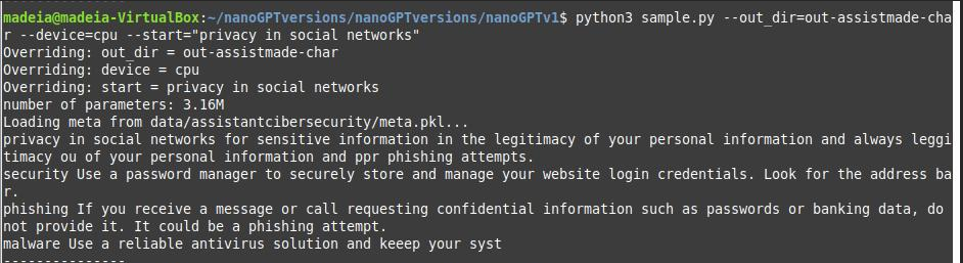
\includegraphics[width=0.65\linewidth]{./rp/12-cp.png} 
              \caption{Resultados de la Prueba 4.1\cite{}}
            \label{figure:Resultado 4 1}  % assign a unique label to each figure 
            \end{figure}
            \item   Prompt = python3 sample.py --out-dir=out-assistmade-char --device=cpu --start="computer security tips"
            \begin{figure}[H]
              \centering % figure is centered on the page
                  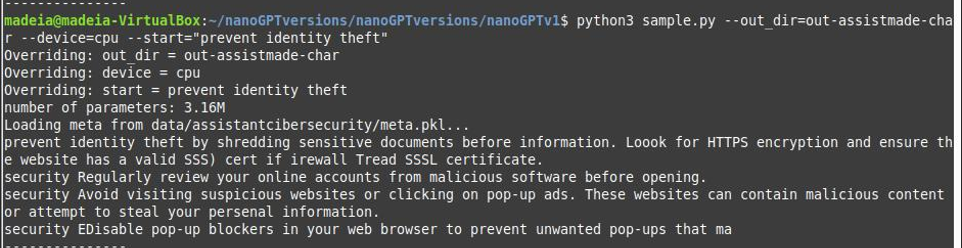
\includegraphics[width=0.65\linewidth]{./rp/13-cp.png} 
              \caption{Resultados de la Prueba 4.2\cite{}}
            \label{figure:Resultado prueba 4 2}  % assign a unique label to each figure 
            \end{figure}
            \item   Prompt = python3 sample.py --out-dir=out-assistmade-char --device=cpu --start="computer security tips"
            \begin{figure}[H]
              \centering % figure is centered on the page
                  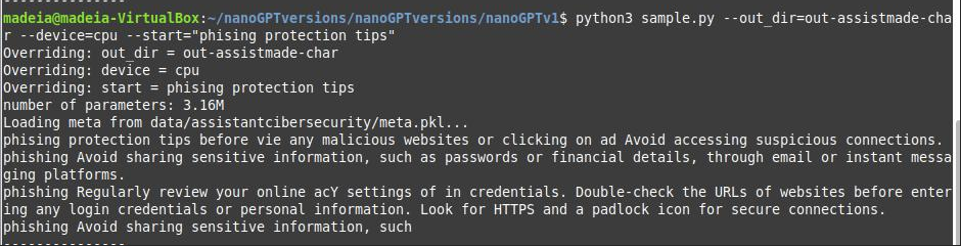
\includegraphics[width=0.65\linewidth]{./rp/14-cp.png} 
              \caption{Resultados de la Prueba 4.3\cite{}}
            \label{figure:Result prueba 4}  % assign a unique label to each figure 
            \end{figure}
    \end{itemize}
%---------------------------------------------------------------------------
%------------------------------------------------------------------------------

 

\chapter{Resultados	y discusión}\label{cap:capitulo5}
%---------------------------------------------------------------------------
\section{Resultados}\label{section:Resultados cap5}


\subsection{Resultados de prompts}\label{section:Análisis de resultados de entrenamiento y resspuestas de clasificación.}

\subsection{Limitantes}\label{section:Limitantes}
%---------------------------------------------------------------------------------------
\section{Discusión }\label{section:Discusión}
%----------------------------------------------------------------------------------------
El rol en la educación se puede empezar debatiendo de manera que se muestre la importancia de la educación en cuanto a promover una cultura tecnológica de manera y la navegación seguras en Internet. ¿Cómo se puede hacer para suplir esa brecha en la educación digital en programas escolares? ¿Qué destrezas y conocimientos deben ser primordial?

Privacidad y protección de los datos, Este es otro punto que se puede debatir iniciando la importancia de la privacidad y la protección de cada persona en el ámbito de la navegación en redes sociales. ¿Qué medidas se debe tomar para así proteger la privacidad de cada uno de los usuarios en línea? ¿Cómo se puede concientizar a mejores prácticas en gestión de datos personales?  

%\chapter{Conclusiones}\label{cap:capitulo6}
%---------------------------------------------------------------------------
%\section{Reflección}\label{seccion:reflection}


\section{Conclusión}\label{seccion:conclusion}

%---------------------------------------------------------------------------
Evaluar cómo es la cultura en temas digitales en Panamá, es una tarea difícil ya que sería comprender su nivel al panorama actual e identificación en áreas de mejoras. Esto incluye una exhaustiva evaluación a la competencia en ámbitos tecnológicos, el acceso a distintas tecnologías, el uso con responsabilidad del Internet y la seguridad en línea de la población. 
Identificar las necesidades y los desafíos que con lleva, durante el tiempo de evaluación, es de mucha importancia. Ya que determinara esas necesidades y desafíos muy específicos en correlación a nuestra cultura digital y la navegación de manera segura en Internet. Esto permitirá que se establezca objetivos de manera clara y de ese modo desarrollar estrategias mucho más adecuada a la hora de abordar.

El Diseñar un modelo para asistir al tema de “seguridad informática”, puede llegar a ser una herramienta muy eficaz para tratar de lograr el objetivo y es concientizar en el ámbito de navegación segura en Internet. NanoGPT podrá brindar ayuda en recomendaciones, recursos educativos, ayudar a comprender riesgos y adoptar buenas prácticas.

Personalizar el asistente, es una tarea complicada y es recomendable crear un diseño. De modo que se pueda adaptar a las necesidades y características de cada uno de los usuarios en Panamá. De manera que pueda incluir la personalización: en cuanto a contenido, el usar ejemplos, escenas que sean relevantes a el contexto local y tomar a consideraración aspecto culturales y lingüísticos.
  

\newpage  

%---------------------------------------------------------------------------
% Bibliografia
% Referencias deben ser agregadas al archivo biblio.bib
\addcontentsline{toc}{chapter}{Bibliografía}
\bibliographystyle{apalike} % Estilo APA
\bibliography{biblio.bib}       % Carga las referencias desde el archivo biblio.bib y crea la sección de Bibliografía  
%---------------------------------------------------------------------------
% Anexos
\appendix  
\clearpage
\addappheadtotoc
\appendixpage
\renewcommand{\thechapter}{\Roman{chapter}}




    
\chapter{Encuesta}
\subsection{Encuesta sobre conciencia digital}\label{section:ResultEn}

\begin{figure}[H]
    \centering % figure is centered on the page
        \includegraphics[width=0.8\linewidth]{./rf/imagen1.png} 
    \caption{Titulo de la Encuesta \cite{}}
   \label{figure:Titulo de encuesta}  % assign a unique label to each figure 
\end{figure}
\begin{figure}[H]
    \centering % figure is centered on the page
          \includegraphics[width=0.8\linewidth]{./rf/imagen2.png} 
    \caption{Primera pregunta de la encuesta \cite{}}
   \label{figure:Resultado1 12} % assign a unique label to each figure
\end{figure}
\begin{figure}[H]
    \centering % figure is centered on the page
          \includegraphics[width=0.8\linewidth]{./rf/imagen3.png} 
    \caption{Segunda pregunta de la encuesta \cite{}}
   \label{figure:Resultado 113} % assign a unique label to each figure
\end{figure}
\begin{figure}[H]
    \centering % figure is centered on the page
          \includegraphics[width=0.8\linewidth]{./rf/imagen4.png} 
    \caption{Tercera pregunta de la encuesta \cite{}}
   \label{figure:Result1ado 5} % assign a unique label to each figure
\end{figure}
\begin{figure}[H]
    \centering % figure is centered on the page
          \includegraphics[width=0.8\linewidth]{./rf/imagen5.png} 
    \caption{Cuarta pregunta de la encuesta \cite{}}
   \label{figure:Res1ultado 6} % assign a unique label to each figure
\end{figure}
\begin{figure}[H]
    \centering % figure is centered on the page
          \includegraphics[width=0.8\linewidth]{./rf/imagen6.png} 
    \caption{Quinta pregunta de la encuesta \cite{}}
   \label{figure:Resul1tado 7} % assign a unique label to each figure
\end{figure}
\begin{figure}[H]
    \centering % figure is centered on the page
          \includegraphics[width=0.8\linewidth]{./rf/imagen7.png} 
    \caption{Sexta pregunta de la encuesta \cite{}}
   \label{figure:Result1ado 8} % assign a unique label to each figure
\end{figure}
\begin{figure}[H]
    \centering % figure is centered on the page
         \includegraphics[width=0.8\linewidth]{./rf/imagen8.png} 
    \caption{Séptima pregunta de la encuesta \cite{}}
   \label{figure:Re1sultado 9} % assign a unique label to each figure
\end{figure}
\begin{figure}[H]
    \centering % figure is centered on the page
         \includegraphics[width=0.8\linewidth]{./rf/imagen9.png} 
    \caption{Octava pregunta de la encuesta \cite{}}
   \label{figure:Resul1tado 10} % assign a unique label to each figure
\end{figure}
\begin{figure}[H]
    \centering % figure is centered on the page
         \includegraphics[width=0.8\linewidth]{./rf/imagen10.png} 
    \caption{Novena pregunta de la encuesta \cite{}}
   \label{figure:Resultado 11} % assign a unique label to each figure
\end{figure}
\begin{figure}[H]
    \centering % figure is centered on the page
         \includegraphics[width=0.8\linewidth]{./rf/imagen11.png} 
    \caption{Décima pregunta de la encuesta \cite{}}
   \label{figure:Resultado 12} % assign a unique label to each figure
\end{figure}
\begin{figure}[H]
    \centering % figure is centered on the page
         \includegraphics[width=0.8\linewidth]{./rf/imagen12.png} 
    \caption{Undécima pregunta de la encuesta \cite{}}
   \label{figure:Resultado 13} % assign a unique label to each figure
\end{figure}
\begin{figure}[H]
    \centering % figure is centered on the page
         \includegraphics[width=0.8\linewidth]{./rf/imagen13.png} 
    \caption{Duodécima pregunta de la encuesta \cite{}}
   \label{figure:Resultado 14} % assign a unique label to each figure
\end{figure}
\begin{figure}[H]
    \centering % figure is centered on the page
         \includegraphics[width=0.8\linewidth]{./rf/imagen14.png} 
    \caption{Décima Tercera pregunta de la encuesta \cite{}}
   \label{figure:Resultado 15} % assign a unique label to each figure
\end{figure}
\begin{figure}[H]
    \centering % figure is centered on the page
         \includegraphics[width=0.8\linewidth]{./rf/imagen15.png} 
    \caption{Décima Cuarta pregunta de la encuesta \cite{}}
   \label{figure:Resultado 16} % assign a unique label to each figure
\end{figure}

\subsection{Resultados de la Encuesta}\label{section:Resultados}

\begin{figure}[H]
    \centering % figure is centered on the page
         \includegraphics[width=0.8\linewidth]{./re/imagen21.png} 
    \caption{Gráfica del Resultado de la Primera pregunta \cite{}}
   \label{figure:Resultado 1} % assign a unique label to each figure
\end{figure}
\begin{figure}[H]
    \centering % figure is centered on the page
         \includegraphics[width=0.8\linewidth]{./re/imagen22.png} 
    \caption{Gráfica del Resultado de la Segunda pregunta \cite{}}
   \label{figure:Resultado 2} % assign a unique label to each figure
\end{figure}
\begin{figure}[H]
    \centering % figure is centered on the page
         \includegraphics[width=0.8\linewidth]{./re/imagen23.png} 
    \caption{Gráfica del Resultado de la Tercera pregunta \cite{}}
   \label{figure:Resultado 3} % assign a unique label to each figure
\end{figure}
\begin{figure}[H]
    \centering % figure is centered on the page
         \includegraphics[width=0.8\linewidth]{./re/imagen24.png} 
    \caption{Gráfica del Resultado de la Cuarta pregunta \cite{}}
   \label{figure:Resultado 4} % assign a unique label to each figure
\end{figure}
\begin{figure}[H]
    \centering % figure is centered on the page
         \includegraphics[width=0.8\linewidth]{./re/imagen25.png} 
    \caption{Gráfica del Resultado de la Quinta pregunta \cite{}}
   \label{figure:Resultado 5} % assign a unique label to each figure
\end{figure}
\begin{figure}[H]
    \centering % figure is centered on the page
         \includegraphics[width=0.8\linewidth]{./re/imagen26.png} 
    \caption{Gráfica del Resultado de la Sexta pregunta \cite{}}
   \label{figure:Resultado 6} % assign a unique label to each figure
\end{figure}
\begin{figure}[H]
    \centering % figure is centered on the page
         \includegraphics[width=0.8\linewidth]{./re/imagen27.png} 
    \caption{Gráfica del Resultado de la Séptima pregunta \cite{}}
   \label{figure:Resultado 7} % assign a unique label to each figure
\end{figure}
\begin{figure}[H]
    \centering % figure is centered on the page
         \includegraphics[width=0.8\linewidth]{./re/imagen28.png} 
    \caption{Gráfica del Resultado de la Octava pregunta \cite{}}
   \label{figure:Resultado 8} % assign a unique label to each figure
\end{figure}
\begin{figure}[H]
    \centering % figure is centered on the page
         \includegraphics[width=0.8\linewidth]{./re/imagen29.png} 
    \caption{Gráfica del Resultado de la Novena pregunta \cite{}}
   \label{figure:Resultado 9} % assign a unique label to each figure
\end{figure}
\begin{figure}[H]
    \centering % figure is centered on the page
         \includegraphics[width=0.8\linewidth]{./re/imagen30.png} 
    \caption{Gráfica del Resultado de la Décima pregunta \cite{}}
   \label{figure:Resulta,do 10} % assign a unique label to each figure
\end{figure}
\begin{figure}[H]
    \centering % figure is centered on the page
         \includegraphics[width=0.8\linewidth]{./re/imagen31.png} 
    \caption{Gráfica del Resultado de la Undécima pregunta \cite{}}
   \label{figure:Result,ado 10} % assign a unique label to each figure
\end{figure}
\begin{figure}[H]
    \centering % figure is centered on the page
         \includegraphics[width=0.8\linewidth]{./re/imagen32.png} 
    \caption{Gráfica del Resultado de la Duodécima pregunta \cite{}}
   \label{figure:Reskultado 10} % assign a unique label to each figure
\end{figure}
\begin{figure}[H]
    \centering % figure is centered on the page
         \includegraphics[width=0.8\linewidth]{./re/imagen33.png} 
    \caption{Gráfica del Resultado de la Décima Tercera pregunta \cite{}}
   \label{figure:Resukltado 10} % assign a unique label to each figure
\end{figure}
\begin{figure}[H]
    \centering % figure is centered on the page
         \includegraphics[width=0.8\linewidth]{./re/imagen34.png} 
    \caption{Gráfica del Resultado de la Décima Cuarta pregunta \cite{}}
   \label{figure:Resultado 10} % assign a unique label to each figure
\end{figure}
%---------------------------------------------------------------------------------------

%---------------------------------------------------------------------------
%---------------------------------------------------------------------------
\end{document}
